\documentclass{article} 
\usepackage{tikz}
\usetikzlibrary{trees}

\begin{document}
	
	\section*{Aufgabe 3}
	
	\subsection*{a)}
	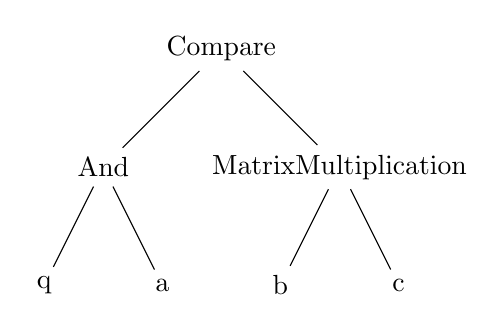
\begin{tikzpicture}[level distance=1.5cm,
	level 1/.style={sibling distance=3cm},
	level 2/.style={sibling distance=1.5cm}
	]
	\node{Compare}
	child {node {And}
		child {node {q}}
		child {node {a}}
	}
	child {node {MatrixMultiplication}
		child {node {b}}
		child {node {c}}
	};
	
	\end{tikzpicture}
	
	\subsection*{b)}
	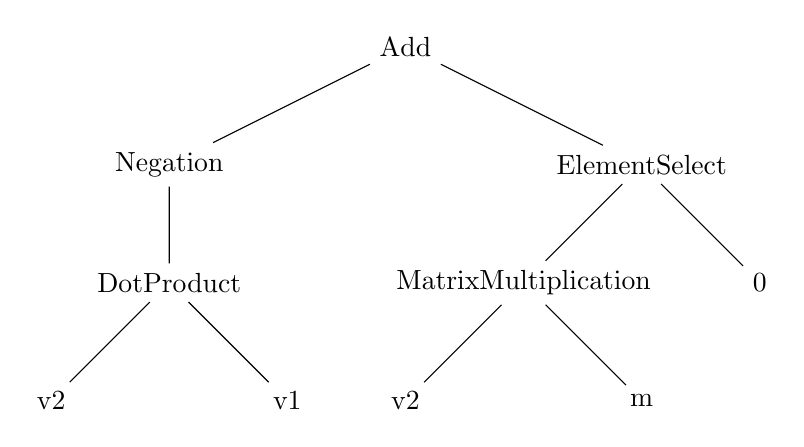
\begin{tikzpicture}[level distance=1.5cm,
	level 1/.style={sibling distance=6cm},
	level 2/.style={sibling distance=3cm}
	]
	\node{Add}
	child {node {Negation}
		child {node {DotProduct}
			child {node {v2}}
			child {node {v1}}		
		}
	}
	child {node {ElementSelect}
		child {node {MatrixMultiplication}
			child {node {v2}}
			child {node {m}}
		}
		child {node {0}}
	};
	
	\end{tikzpicture}
	
\end{document}